\chapter{Estado da arte}
\label{cap_estado_arte}

Neste capítulo, será feita uma exposição do estado da arte das tecnologias relacionadas com o tema ou relevantes para o projeto, assim como trabalhos relacionados, quer no mesmo tema ou envolvente - algoritmos relevantes para o desenvolvimento -, procurando plantar uma base para o trabalho realizado e futuro, entendendo o que já foi explorado e o que está para vir em alguns casos.
O capítulo começa com uma apresentação sobre \acrshort{ocr} que será a tecnologia pilar do trabalho (\ref{sec_ocr}), seguido por uma exploração de processos de melhoria dos resultados de reconhecimento usando pré (\ref{sec_pre_proc_ocr}) e pós processamento (\ref{sec_pos_proc_ocr}). Procede-se o tema de segmentação de documentos (\ref{sec_segmentacao_docs}), terminando com o estudo de trabalho relacionado (\ref{sec_trab_relacionado}).

% pequeno resumo dos temas que serão tratados


\section{Reconhecimento ótico de caracteres}
\label{sec_ocr}


\subsection{Introdução}

O reconhecimento ótico de caracteres é a tecnologia base do projeto proposto, estando presente em qualquer instância ou caso de estudo que será explorado, inclusive em exceções que não necessitam a aplicação de reconhecimento de caracteres, como ficheiros do género \textbf{hOCR},  pois estes já são um produto de \acrshort{ocr}.

Na sua essência e como o nome indica, software de reconhecimento ótico de caracteres permitem a deteção e transcrição de texto a partir de imagens, de forma automática e autónoma. Utilizando esta habilidade, abriu-se a possibilidade de tornar os documentos digitalizados ao longo do tempo numa fonte mais útil de informação: navegada, consultada e editada mais facilmente, visto estes serem na maioria dos casos, digitalizados na forma de imagens. A adição do conteúdo destes documentos através da sua transcrição, mesmo que apenas parcialmente correta, permite a adição de, por exemplo, meta-dados ou palavras chaves que auxiliam a sua indexação. 




\subsection{Breve história e evolução}

\cite{10.5555/1074100.1074664} e \cite{6993174} apresentam a história do reconhecimento ótico de caracteres desde a conceção do seu ideal no século XIX, como uma tecnologia para auxílio de pessoas com impedimentos na leitura, até aos pontos alcançados na última década onde até escrita humana se tornou num desafio, até certo ponto, conquistável.
As primeiras instâncias de reconhecimento óptico realizado por máquinas deu-se no final do séc. XIX, mais especificamente em 1870 por Charles R. Carey  com a criação de um scanner de retina, mas é necessário ir até meio do século seguinte e pela consequente evolução que decorreu nesta área, para a subárea de reconhecimento de caracteres começar a ver a sua comercialização com a invenção de David Shepard: GISMO, um sistema simples capaz de reconhecer texto .

A génese desta tecnologia começou num formato bastante limitado, sendo capaz apenas de reconhecer um conjunto muito limitado de caracteres de uma fonte específica a um ritmo de 1 caráter por minuto, isto em condições de input bem controladas (papel sem ruído, apenas com o texto a ser reconhecido). Esta é considerada por \cite{6993174} como a primeira geração de \acrshort{ocr}.

A segunda geração começa a dar os primeiros passos no processamento de escrita humana, como é exemplo o \textit{IBM 1287} na década de 60.

A terceira geração, nas décadas de 70 e 80, introduziu um maior foco no processamento da escrita humana e na capacidade de lidar com problemas na imagem original.

A quarta geração tornou-se capaz de tratar documentos complexos com misturas entre texto e imagens, assim como qualidades de inputs menos favoráveis, documentos com cor e mais precisão com texto manuscrito.

Atualmente com a evolução das técnicas de pré processamento, assim como os algoritmos de reconhecimento e a ascensão da inteligência artificial \citep{9183326}, a precisão e flexibilidade dos softwares de \acrshort{ocr} são capazes de, até em imagens de paisagens, segmentar e reconhecer texto localmente de forma automática e com pouco pré processamento. Além disso, embora o foco anteriormente era em software \acrshort{ocr} pago e dedicado a um tipo específico de documentos, a implementação de softwares mais geral e de uso aberto tem-se tornado mais vulgar.
Em algumas instâncias complexas - documento complexo e linguagem com caracteres fora do latim -, já existe tecnologia capaz de obter taxas de acerto acima dos 95\% mesmo para texto escrito à mão \citep{9183326}.   


\subsection{Processo OCR}
Um software \acrshort{ocr} pode ter reconhecimento online ou offline \citep{10.5555/1074100.1074664}\citep{6993174}.  O primeiro é reconhecimento em tempo real, em que usualmente o input é obtido num dispositivo dedicado como um tablet digitalizador,  no formato de um conjunto de coordenadas, podendo portanto ser mais preciso a custo de menor flexibilidade na entrada. O mais comum, método offline, recebe como um input por norma uma imagem com o documento finalizado. O bitmap desta imagem será utilizado como alvo do reconhecimento de caracteres. O uso deste último método, com tipo de entrada menos controlado, exige uma fase de pré processamento mais minuciosa do que o reconhecimento online.

Neste trabalho, o foco será dado ao reconhecimento offline por ser o mais comum e aquele que permite o tratamento de documentos pré digitalizados.
Este pode ser geralmente divido em 6 partes:

\begin{wrapfigure}{r}{0.3\textwidth}	
	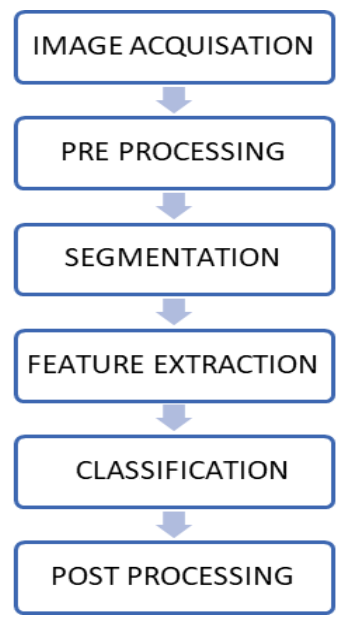
\includegraphics[width=0.3\textwidth]{images/ilustracoes/processo_ocr.png}
\end{wrapfigure}
\noindent
\begin{itemize}
    \item \textbf{Aquisição de input} : imagem a ser reconhecida, incluindo algoritmos de compressão do próprio formato guardado.
    \item  \textbf{Pré processamento} : técnicas de manipulação do input para melhorar resultado de \acrshort{ocr}
    \item \textbf{Segmentação} : segmentação do input, a vários níveis, de modo a isolar o melhor possível os conteúdos relevantes, i.e. o texto.
    \item \textbf{Extração de características} : processo de reconhecimento de características dos caracteres isolados.
    \item \textbf{Classificação} : utilizando as características calculadas é feita a decisão sobre a sua identidade.
    \item \textbf{Pós processamento} : técnicas para melhoria do resultado como, por exemplo, a correção de erros ortográficos. Por vezes pode alterar o documento original se a \gls{ground truth} já contiver estes erros.
\end{itemize}
\noindent

O \textbf{Pré Processamento} é um passo essencial para o aumento do acerto do reconhecimento de texto, sendo que ele pretende remover imperfeições do input como: baixo contraste das linhas, texto mal delimitado, ruído de imagem, orientação do documento ou do texto (principalmente manuscrito). Em alguns casos mais complexos, com ajuda de inteligência artificial, também é possível a reposição de partes parciais de uma imagem que foram perdidas, ou remoção de elementos como \textit{watermarks}.

A \textbf{Segmentação} é usada para isolar o conteúdo útil do resto da imagem podendo envolver vários passos como: segmentação da página para separar texto do resto do conteúdo; segmentação de caracteres, com o intuito de os separar em caracteres individuais, algo que é especialmente difícil com escrita à mão devido à tendência  em criar ligações entre caracteres ou mesmo de os unir; tratamento e normalização dos caracteres isolados - normalização do tamanho, filtração morfológica.

A \textbf{Extração de Características} (Feature Extraction) trata-se do processo de deteção e cálculo das características dos caracteres, para a criação do classificador (dependendo da arquitetura) e anotação do que distingue o caráter alvo. Este processo é possivelmente o mais aberto para variações e que, juntamente com o classificador, mais influencia o resultado. Diferentes técnicas de extração de características e \textbf{Classificação} são utilizadas e foram estudadas durante as últimas décadas: desde \textit{template matching} \citep{10.5555/1074100.1074664} onde são usados algoritmos para cálculo de similaridade entre um template e o alvo, a segmentação de características, como presença de loops ou traços verticais longos  \citep{10.5555/1074100.1074664}, ou distribuições de pixeis \citep{9183326}. 
Para texto humano, este processo torna-se ainda mais complexo devido à necessidade  de lidar com múltiplos caracteres  invés de singulares. 
A classificação passava por um processo de comparação do valor das características calculado com diferentes templates porém, mais recentemente, o uso de estratégias no ramo de machine learning são mais comuns: redes neuronais, support vector machines e k- nearest neighbor; são alguns dos modelos mais utilizados \citep{9183326} \cite{6993174}. Por vezes, o classificador utiliza conhecimento do léxico de uma linguagem para ajudar na sua classificação, sendo que documentos com linguagem desatualizada poderão sofrer nesse caso.

O \textbf{Pós Processamento} é responsável pelo tratamento do output, responsável por mitigar ou corrigir alguns erros do reconhecimento, desde correções ortográficas a posicionamento na página \citep{9183326}.

Este trabalho irá ter como foco principal as secções de pré e pós processamento, e segmentação, na procura de aumentar a eficácia do reconhecimento e da organização dos resultados.



\subsection{Desafios}
\label{ocr_desafios}

\newglossaryentry{ground truth}{
name= ground truth,
description={Em OCR, este é o nome dado ao conteúdo do documento original. Usualmente apenas o conteúdo textual é considerado.}
}

Com a evolução da tecnologia, os problemas foram mudando de foco, tendo passado por um longo período em que a maior prioridade era a capacidade de reconhecimento de caracteres para além de um escopo limitado, tanto em termos de identidade quanto estilo, para a capacidade de tratar a imagem de forma a que o reconhecimento tenha uma maior taxa de acerto \citep{4283429}.
Alguns dos maiores desafios atualmente para \acrshort{ocr} são:
\begin{itemize}
    \item \textbf{documento original} : danos  no objeto; texto ilegível ou com um tipo de letra muito complexo; linguagem desatualizada; estrutura complexa; inclinação do texto; distorções da página.
    \item \textbf{imagem} : má iluminação; múltiplas páginas com diferentes orientações; baixa resolução; pouco contraste; ruído.
    \item \textbf{classificador ou extrator de features} não adequado para uma dada linguagem.
    \item \textbf{resultado} : validação quando não se tem a \gls{ground truth} disponível
\end{itemize}

Dentro destes, o processamento de estruturas complexas será o foco principal e o expectável maior contributo deste trabalho.


\subsection{Tecnologia}

\newglossaryentry{codec}
{
    name=codec,
    description={Algoritmo de compressão com o propósito de diminuir a dimensão de uma entidade.}
}

\newacronym{ml}{ML}{Machine Learning}

Presentemente, com a proliferação permitida pela internet e a globalização, a disponibilização de ferramentas de \acrshort{ocr}, anteriormente primariamente privilégio de instituições ou empresas, como bancos \citep{10.5555/1074100.1074664}, tornou-se trivial, acessível através de itens do dia a dia como um computador ou telemóvel de forma gratuita, ex.: Google Lens.

Alguns destes softwares que serão utilizados neste trabalho são:
\begin{itemize}
    \item \textbf{Tesseract} 
    \item \textbf{Keras-OCR}
    \item \textbf{PaddleOCR}
\end{itemize}

Os resultados deste tipo software podem ser genericamente descritos como uma lista de caixas, delimitadoras de texto, com conteúdo, i.e. o texto nela contido e, por norma, um nível de confiança no reconhecimento desse texto.

No caso do \textbf{Tesseract} \citep{tesseract_doc}, dentro das várias formas que os resultados podem ser apresentados, a lista de caixas pode ser interpretada como uma árvore de blocos, em que cada nível corresponde a um tipo de estrutura no documento: página $\longrightarrow$ bloco $\longrightarrow$ parágrafo $\longrightarrow$ linha $\longrightarrow$ texto. 

Usando \textbf{PaddleOCR} \citep{paddle_doc}, os resultados são mais simples, divididos apenas pelas linhas de texto detetado.

Já o \textbf{Keras-OCR} \citep{keras_doc} lista um conjunto de caixas em que cada contém uma palavra reconhecida.

Uma outra característica que o \textbf{Tesseract} tem é a capacidade de reconhecer, com nível de acerto variável, outros elementos relevantes de um documento, como imagens ou delimitadores. Isto pode, por outro lado, causar erros na interpretação dos resultados por sobreposição ou multiplicação da quantidade de caixas.  Além disso o \textbf{Tesseract} permite bastantes configurações como: léxico esperado; modo de segmentação; reconhecimento de espaços em branco; etc.

O output deste tipo de software pode ainda ser processado para tomar diversas formas: formatos que apenas retém o conteúdo como texto simples ou markdown;  formatos que mantém informação sobre os blocos detetados, como hOCR.

A validação do output é na maioria dos casos medida a partir da comparação com a \gls{ground truth}, o que limita a capacidade de testar e treinar (no caso de \acrshort{ml} supervisionado) modelos visto que os datasets tem de ser criados de forma minuciosa e consumidora de tempo.

Além dos softwares de reconhecimento, é preciso ter atenção ao tipo dos ficheiros de entrada. Estes são usualmente imagens e, dependendo do tipo de \gls{codec} destes, os algoritmos de compressão aplicados poderão diminuir a qualidade de imagem, como é o caso de formatos \textit{lossy} como \textbf{JPEG}, potencialmente diminuindo o acerto do reconhecimento do texto. \cite{7367194}, no seu estudo demonstra que mesmo entre diferentes tipos de \textit{lossy} \gls{codec} o seu impacto pode variar significativamente nos resultados de \acrshort{ocr}, sendo que o formato \textbf{JPEG}, um dos mais populares, resultou nas menores taxas de sucesso.



\section{Pré Processamento para OCR}
\label{sec_pre_proc_ocr}

\newacronym{dpi}{DPI}{dots per inch}
\newacronym{cnn}{CNN}{Convolutional Neural Network}
\newacronym{gan}{GAN}{Generative Adversarial Network}
\newacronym{psnr}{PSNR}{Peak signal-to-noise ratio}
\newacronym{ssim}{SSIM}{Structural similarity index measure}

Como foi listado na secção \ref{ocr_desafios}, existe uma diversa quantidade de defeitos que os documentos originais e as imagens digitalizadas destes podem ter e cuja presença pode afetar negativamente os resultados de software de \acrshort{ocr}. 
O pré processamento pode ser considerado como uma fase de tratamento de imagem para remover estes problemas que deterioram o reconhecimento de texto. De forma a entender os diferentes métodos utilizados e a sua evolução para o presente, foram selecionados os estudos:  \citep{4283429},\citep{5277501},\citep{9187695},\citep{8545609},\citep{9791698},\citep{8368720},\citep{8269967}.

Entre o grande leque de diferentes algoritmos e tratamentos que podem ser aplicados nas imagens, em geral, estes podem ser segmentados nos mais comuns \citep{9791698}:
\begin{itemize}
    \item \textbf{binarização/thresholding da imagem} : processo de normalização dos pixeis para um de dois valores, mediante um determinado limiar
    \item \textbf{remoção de ruído} : algoritmos para retirar degradações ou sujidades da imagem através de processos como, por exemplo, suavização da imagem calculando para cada pixel o valor médio da sua vizinhança
    \item \textbf{correções de texto} : alguns casos deste são texto que apresenta um ângulo de rotação, texto com inclinação, distorções locais no texto, \textit{watermarks}
    \item \textbf{super-resolução} : aumentar a resolução da imagem, consequentemente aumentando o seu \acrshort{dpi}
    \item \textbf{foco da imagem} : acentuação das arestas, diminuir desfocagem
    \item \textbf{transformações morfológicas} : operações sobre a imagem de modo a provocar maior contraste do conteúdo, ou permitir melhor distinção das características, ex.: dilatação do texto para tornar mais fácil a distinção entre regiões com e sem texto.
\end{itemize}

Para \textbf{binarização}, o objetivo principal é distinguir o texto do resto da imagem, daí a alocação dos pixeis para 1 de dois valores. Este processo é distinguido principalmente entre o uso de \textit{thresholding} global ou local (ou adaptativo), sendo que o global implica um cálculo das características estatísticas locais dentro da imagem, e é mais adequado para o tratamento de imagens com cor, ou com variações de intensidade dispersas pela imagem \citep{9791698}. Alguns dos algoritmos mais comuns são comparados por \cite{9187695}, onde é evidente a dependência destes nas condições do documento original e da imagem. Um exemplo apresentado demonstra como, numa imagem com uma mancha escura (com o texto ainda distinguível), o algoritmo de Otsu conseguiu gerar uma imagem com pouco ruído e bom contraste, mas a zona da mancha fica completamente preta, comparado ao algoritmo de Niblack que, embora com mais ruído, recuperou algum texto dentro da mancha.

A \textbf{remoção de ruído} é possivelmente a área com mais alternativas possíveis e das que mais afeta o resultado do reconhecimento por, a nível de pixeis, o ruído interferir com a composição dos caracteres ou criar acumulações de informação extra que serão mal identificadas pelos softwares, como notado por \cite{4283429}. 
O ruído nas imagens pode ser de vários tipos, o que dificulta a forma de o detetar e tratar. 
Alguns dos outros tratamentos, como a binarização, transformações morfológicas e alguns tipos de super-resolução, também tratam desta questão mesmo não sendo o seu foco principal.  Da mesma forma, alguns dos filtros utilizados podem ter outros resultados como o aumento do contraste ou eliminação de distorções.
Alguns dos tratamentos mais comuns do ruído são\citep{9791698}\citep{8269967}\citep{4283429}:
\begin{itemize}
    \item filtro Gaussiano
    \item médias não locais
    \item suavização com filtro de mínimos locais
    \item suavização com filtro Wiener
\end{itemize}
Vários destes métodos resultam  tanto na acentuação das arestas do texto, como na remoção de lixo ou ruído à sua volta,  recuperando o \textbf{foco da imagem}.

A \textbf{correção de texto} necessita, ao contrário dos outros processos que podem, mesmo sem uma análise prévia do estado da imagem, melhorar o reconhecimento de texto; de uma análise prévia visto que, por exemplo, não se pode aplicar uma rotação na imagem sem saber o ângulo de orientação inicial desta. 
\cite{4283429} faz uma apresentação convincente do efeito de uma rotação de ângulo 15º no reconhecimento do Tesseract, o que impediu o reconhecimento.
O método proposto passa pelo computação de uma linha que afete a margem na extremidade esquerda do texto, de modo a calcular a sua inclinação relativa à margem da imagem e assim descobrir o ângulo de rotação do texto.
No espectro mais limitado da sua proposta, devido à sua localidade nos documentos, \cite{4283429} discute distorções nos documentos como curvaturas resultantes da bainha de um livro. Aqui, em traços gerais, a linha de curvatura do texto é detetada, com a qual é criado um quadrilátero da área afetada, onde será, de acordo com o nível de curvatura na projeção sobre a linha, realizada a correção.
Em ambos os casos, os resultados demonstrados para casos de grande deformação, os algoritmos propostos conseguiram tornar a completa falha de reconhecimento para taxas de acerto dentro dos 99\%.

A aplicação de \textbf{super-resolução} procura auxiliar o processo de reconhecimento ao melhorar a qualidade de imagens de baixa resolução, i.e. aumentar os seus \acrshort{dpi} e tornar os caracteres mais reconhecíveis. 
Entre os vários algoritmos utilizados para este propósito, o uso de interpolação tendia a ser o mais comum, porém nem sempre os resultados eram satisfatórios, resultando em imagens transformadas serem desfocadas, ou com os defeitos originais acentuados, especialmente quando o salto era feito a partir de imagens com \acrshort{dpi} baixo - 100 ou menos \citep{8545609}. No entanto, com os avanços na área das redes neuronais, em particular na categoria de imagens naturais, modelos como \acrshort{cnn} \citep{8368720},\citep{8545609} trouxeram uma nova forma treinar algoritmos para tratar imagens de forma adaptativa e com resultados muito melhores do que os algoritmos bem estabelecidos para este problema. Um dos pontos negativos deste tipo de redes é que a criação de datasets de treino é um processo demorado, sendo que para cada imagem de treino (degradada), é necessário uma imagem par com o resultado ideal para validação do resultado. Adicionalmente estes datasets têm de ter casos com características dispersas o suficiente para permitir uma boa generalização do modelo. Um outro modelo que tem vindo a emergir são as \acrshort{gan} que, invés de utilizarem uma única rede para gerar conteúdo que depois será validado em cada iteração do treino, utilizam duas redes que competem diretamente: a geradora que tenta transformar imagens de modo a enganar o discriminador, e este que tenta entender se a imagem de input é a imagem original ou se foi gerada. \cite{9187695} propõe um modelo deste género que demonstra a sua superioridade tanto em relação a algoritmos baseados em regras, como de modelos baseados em \acrshort{cnn}.

As \textbf{transformações morfológicas} são compostas por vários métodos e propósitos diferentes, nem sempre com o intuito de melhorar a qualidade da imagem, mas para acentuar certas características desta. Por exemplo, técnicas como a dilatação podem ser utilizadas para acentuar regiões de texto de forma a ser possível separar o texto do resto. Por outro lado, técnicas de deteção de arestas, erosão ou \textit{thinning}, diminuem o tamanho dos elementos da imagem, podendo simplificar os caracteres, tornando o seu reconhecimento, ou das suas características (como loops) mais evidentes \citep{9791698}.

Estes diferentes tipos de tratamento podem, na grande maioria dos casos, complementar-se mutuamente e, é costume - inclusive nos estudos referenciados - a criação de pipelines de pré processamento que aplicam estes vários tratamentos de forma sequencial. No entanto, como estes diferentes tratamentos impactam diretamente os dados de input para reconhecimento, nem sempre são benéficos e têm de ser escolhidos com cuidado consoante o estado do sujeito.  \cite{8269967} demonstra precisamente isto mostrando, por exemplo, que a aplicação de um filtro Gaussiano para a redução de ruído num caso de teste reduziu a taxa de acerto do Tesseract para menos de 1 terço comparado ao resultado sem pré processamento. 
Isto naturalmente dificulta a criação de pipelines automáticas de pré processamento. Nesse mesmo estudo, é proposto o uso de uma \acrshort{cnn} que, consoante um número limitado de classes que representam combinações de técnicas de pré processamento, decide a melhor para uma dada imagem. Esta solução resultou numa melhoria considerável, principalmente para o reconhecimento do Tesseract e, mais interessante, a tendência para certas combinações de técnicas com: binarização escolhida \~90\% das vezes, redução de ruído 35\% e acentuação de contrastes 34\%.
Como mencionado anteriormente, os avanços no tratamento de imagem com uso de modelos de Deep Learning vêm trazer, quando suficientemente generalizados, um método ubíquo para a realização destes vários tratamentos de forma adaptativa. \cite{9187695} com a \acrshort{gan} proposta, demonstra resultados no tratamento de ruído, focagem, binarização e remoção de \textit{watermarks} excelentes, mesmo tendo em conta que o foco principal do modelo era o aumento da resolução da imagem original. 

\subsubsection{Métricas de avaliação}
No ato de  pré processamento, as métricas de avaliação são muitas das vezes subjetivas visto, em geral, se tratar de tratamento de imagem e nem sempre haver uma versão não degradada das imagens dos documentos. No caso de haver essa versão prístina, algumas das métricas mais comuns para testar o tratamento de modelos ou algoritmos são: \acrshort{psnr}, que compara o ruído na imagem tratada comparativamente com a original, sendo que valores maiores tendem a significar melhores resultados; e \acrshort{ssim}, que tenta ter em conta as similaridades das vizinhanças na imagem, assim como outros aspetos mais relativos a cor e luminosidade, imagens idênticas terão valor 1. Não havendo a possibilidade de testar com uma imagem base, pode-se avaliar o efeito do pré processamento através da variação dos resultados do output ou do pós processamento.


\section{Pós Processamento para OCR}
\label{sec_pos_proc_ocr}
\newacronym{nlp}{NLP}{Natural Language Processing}
\newacronym{lstm}{LSTM}{Long Short Term Memory}

Na generalidade, o tratamento dos resultados de \acrshort{ocr} ronda em torno das correções sob o texto resultante. Estas correções procuram corrigir erros ortográficos, texto irreconhecível, ou sem sentido (caracteres lixo ou ruído reconhecido).

Correções a nível dos blocos/caixas que englobam o texto reconhecido, são mais orientadas ao tipo de documento e ao seu contexto e serão analisadas com mais atenção nas secções seguintes.

\cite{10.1145/3453476} apresentam um estudo extremamente compreensivo e extenso sobre o estado da arte e o impacto do pós processamento no texto resultante de \acrshort{ocr}.

Neste estudo, é apresentado primeiramente a importância deste tratamento de texto, não só para aumentar a qualidade das aplicações que o utilizam, exemplo dado no caso de \acrshort{nlp}: onde taxas de erro por volta dos 7\% podem mostrar reduções na qualidade da análise de sentimento de até 30\%; mas também no próprio processo de navegação e procura por documentos transcritos por \acrshort{ocr} : em alguns exemplos os erros de texto não permitiram uma indexação ou reconhecimento de termos de pesquisa correta, não sendo devolvidos na procura.

Os dois principais erros de texto reconhecido são:
\begin{itemize}
    \item \textbf{não palavra} : quando uma palavra reconhecida pelo motor de \acrshort{ocr} não se encontra no léxico conhecido
    \item \textbf{palavra real} : a palavra reconhecida pertence ao léxico conhecido, porém difere da \gls{ground truth}
\end{itemize}
Dentre estes dois tipos de erro, o primeiro é consideravelmente mais fácil de detetar e potencialmente corrigir, visto o segundo necessitar de informação adicional, quer seja esta a \gls{ground truth} do documento - o que é raro -, ou uma análise da palavra dentro do seu contexto.

O estudo segue então para a secção das técnicas de pós processamento. Estas são separadas em dois tipos principais: \textbf{manuais} e \textbf{(semi-)automáticas}.

As técnicas \textbf{manuais} entendem total ação humana e são normalmente dirigidas para projetos mais sensíveis a erros mas que, pela necessidade desta mão de obra, são naturalmente mais custosos, demorados e raros. São casos destes, projetos de transcrição de documentos antigos, como é dado exemplo o projeto da biblioteca nacional da Austrália na correção de jornais históricos.
Alguns outros casos destas técnicas descritos servem mais para o propósito de avaliação de algoritmos ou criação de casos de teste.

As técnicas \textbf{(semi-)automáticas} podem ser agrupadas em dois tipos: \textbf{tratamento de palavras isoladas}, e \textbf{dependentes de contexto}. Dentro destas, o tratamento de palavras isoladas é focado na correção de problemas de 'não palavra', enquanto as dependentes de contexto procuram resolver os dois tipos de problemas.


Dentro das diferentes técnicas baseadas nas \textbf{palavras isoladas}, algumas características servem como fundamentos dos algoritmos:
\begin{itemize}
    \item \textbf{Léxico conhecido}
    \item \textbf{Confiança do reconhecimento}
    \item \textbf{Frequência de utilização de uma palavra, no documento, ou globalmente}
    \item \textbf{Similaridade da palavra errada com as conhecidas no léxico}
\end{itemize}
Entre algumas destas técnicas, são realçadas:

\subsubsection{Junção de Outputs de OCR}

A junção de outputs de OCR visa a escolher entre diferentes resultados para uma dada sequência de palavras, com características distintas (nível de confiança no reconhecimento, quantidade de erros,etc.), e escolher dentro destas ou numa sua mistura, o output final.

Numa 1º fase, os outputs são então obtidos, onde para isto várias propostas foram feitas, com as principais sendo: 
\begin{itemize}
    \item Usando o mesmo motor OCR, fazer vários reconhecimentos de um mesmo trecho de texto
    \item Usando o mesmo motor OCR, fazer vários reconhecimentos de um mesmo trecho de texto, com parâmetros diferentes ou tratamento de imagem diferente
    \item Usando múltiplos motores OCR, fazer vários reconhecimentos de um mesmo trecho de texto
\end{itemize}

Numa 2º fase, estes diferentes outputs têm de ser alinhados de forma a poderem ser comparados palavra a palavra. Para isto, algoritmos sob grafos são comuns.

Por último, utilizando um decisor, o output final é escolhido. Este decisor pode tomar várias formas como: modelos de votação, cálculo de similaridade com léxico, modelos \acrshort{lstm}.

Embora esta técnica geralmente resulte em resultados melhores do que o reconhecimento simples, exige um maior gasto computacional, assim como do facto de estar limitado ao dicionário conhecido.

\subsubsection{Vias lexicais}
Uma outra visão sobre o tratamento do texto, é na procura das palavras mais similares à não palavra detetada e, dentro destas, decidir qual a que tem maior potencial para a substituir. Este cálculo de similaridade pode ser realizado de várias formas, sendo das mais comuns: a distância de Levenshtein, onde se calcula o número de operações mínimas - inserção, remoção ou substituição - a realizar numa palavra para obter outra; variações deste algoritmo; e distância entre n-gramas, que envolve a quantidade de conjuntos de palavras em comum entre as duas palavras comparadas.

Como no caso anterior, estas vias continuam limitadas pelo léxico conhecido, sendo que muito do estudo é dedicado à criação de dicionários mais abrangentes ou adaptados ao documento, ex.: pegando em palavras chaves do documento ou de um tema e criar um dicionário com as páginas mais relevantes de uma pesquisa feita sobre estes.

\subsubsection{Modelos de erro e Máquinas de estado finitas com pesos}
Os modelos de erro procuram calcular as probabilidades sob as operações nos caracteres da palavra errada e, a partir destes e do léxico conhecido, decidir qual o melhor candidato para substituição.

Estes modelos de erro podem ser complementados por máquinas de estados finitas com pesos. Os modelos de erro são utilizados para a escolha de candidatos para substituir o erro, e os pesos da máquina são dependentes de características entre os candidatos e a palavra errada como: comprimento, semelhança, entre outras.

\subsubsection{Modelos de linguagem baseados em tópicos}
No decisão de candidatos para substituição da palavra errada, outros trabalhos sugeriram o uso de contexto do documento de forma parcial, i.e. calcular o tópico do documento a partir da análise deste e utilizar esta informação como um variável extra nas fases de decisão de candidatos. Assim, palavras que sejam numa perspetiva global mais raras não serão tão facilmente descartadas como nos métodos anteriores.

Tal envolve no entanto um processo de decisão sobre quais os tópicos que existem, e a adaptação do léxico para criar correspondências entre as palavras e estes dados tópicos.

\hspace{10pt}

\par Dentro dos métodos \textbf{dependentes de contexto}, são notados os ramos:

\subsubsection{Modelos de linguagem}
\newglossaryentry{word embeddings}
{
name = word embeddings,
description={Forma de vetorização de uma palavra. O vetor de uma palavra representa os seus valores num conjunto de características.}
}

Partindo como base os modelos anteriormente descritos, complementam os modelos com o cálculo da probabilidade de distribuição de sequências de palavras, sendo estas parte do documento. Assim, para cada palavra, utilizando os seus vizinhos, será calculada a probabilidade daquela sequência ocorrer. Este cálculo pode ser calculado utilizando léxicos já definidos, ou complementando estes com as frequências dos n-gramas de palavras dentro do documento. Estes modelos caem dentro do ramo estatístico.

Um outro tipo é conseguido através de redes neuronais que a partir do texto criam \gls{word embeddings}, o que permite calcular a similaridade entre palavras tendo em conta as suas características. Com esta habilidade, as sequências de palavras do texto reconhecido podem ser sujeitas ao cálculo da probabilidade de ocorrerem e, caso este seja muito baixo, poderá ser sinal de um erro de palavra real.

\subsubsection{Machine Learning baseado em características}

Neste caso, o contexto é utilizado dentro de uma quantidade de características mais limitado mas também mais robusto do que na alternativa anterior. Algumas destas características tendem a ser:
\begin{itemize}
    \item Frequência da palavra - nos casos de treino e no próprio documento
    \item Frequência dos ngramas com a palavra -  nos casos de treino e no próprio documento
    \item Peso de confusão - conseguido através dos casos de treino
    \item Confiança do motor OCR na palavra
\end{itemize}

\subsubsection{Seq2Seq - Sequência para Sequência}

Esta alternativa, tem como noção que este problema de correção é uma questão que pode ser resolvida por tradução máquina, correspondendo à transformação numa sequência de palavras, numa outra idêntica ou semelhante, na mesma linguagem.

Estes modelos, ao contrário dos mencionados de modelos de linguagem - que recebendo uma sequência de palavras analisavam a probabilidade de uma outra ser a próxima na sequência, ou sugeriam a próxima palavra -, recebem uma sequência de palavras e devolvem também uma sequência de palavras.

\hspace{10pt}

O estudo termina com uma análise das tendências destas diferentes áreas, onde se pode notar uma aderência maior para tecnologias de inteligência artificial, juntamente com a tendência para a união dos dois ramos de tratamento de texto (semi-)automático nas soluções.


\subsubsection{Métricas de avaliação}
Como acontece no caso do pré processamento, o pós processamento necessita de uma \gls{ground truth} para poder ser avaliado. Contra esta, diferentes medições podem ser feitas, como a percentagem de caracteres ou palavras totais nos dois textos, ou a taxa de acerto tendo em conta alinhamento dos textos. Algumas características como a quantidade de \textit{whitespaces} e indentação também podem ser relevantes para certos tipos de documentos. A quantidade de substituições realizadas, mais propriamente de palavras não reais, também pode ser importante para avaliar o software de reconhecimento, embora este erro possa ser resultado de um léxico não apropriado para o documento, ex.: documentos históricos. 

\section{Segmentação de documentos}
\label{sec_segmentacao_docs}

A segmentação de documentos é um processo que visa decompor o documento nas suas várias secções ou elementos. A sua aplicação pode variar dependendo do objetivo concebido: separação do texto de elementos não texto, retirando informação prejudicial para \acrshort{ocr}; divisão do conteúdo do documento em várias secções para que possam ser analisadas ou extraídas isoladamente. Por este mesmo motivo, estes processo tem aplicabilidade tanto antes como depois de feito o reconhecimento de texto.

\cite{ESKENAZI20171} faz um estudo compreensivo sobre as diferentes metodologias de segmentação de documentos, apresentando as suas diferentes características, evolução e tendências. 
As diferentes técnicas podem ser dividas de forma comum como: 
\begin{itemize}
    \item \textbf{top-down} : divisão a partir da página em blocos mais pequenos
    \item \textbf{bottom-up} : a partir de uma escala mais pequena, ex.: pixeis, componentes conectadas; os elementos são aglomerados em conjuntos maiores até completar a página
    \item \textbf{hibrído}
\end{itemize}

O estudo decide invés seguir por uma divisão em 3 grupos de acordo com a evolução da capacidade dos algoritmos de segmentar diferentes tipos de documentos.
\begin{itemize}
    \item \textbf{Dedicado a um esquema (layout) específico}
    \item \textbf{Capaz de lidar com layouts descritos por um conjunto de parâmetros}
    \item \textbf{Layout potencialmente não restrito}
\end{itemize}

\subsubsection{Algoritmos dedicados a um layout específico}

Estes algoritmos, têm como objetivo a segmentação de um dado tipo de esquema. Estes tendem a ser mais rápidos e, embora os menos versáteis, apresentam para o seu tipo de alvo resultados difíceis de superar. Dentro destes, existem 3 ramos principais de algoritmos. 

O primeiro, são os algoritmos que assumem as características do esquema e, usando estas, criam gramáticas que os descrevem, ou criam perfis do esquema que são projetados nas imagens de input para aplicação de heurísticas de alinhamento e análises probabilísticas para deteção de erros ou desalinhamentos

O segundo ramo, foca-se no uso de filtros para realce de regiões de um layout. Estes são normalmente utilizados para documentos em que as linhas do texto sejam retas e horizontalmente alinhadas. Os casos mais frequentes destes algoritmos aplicam morfologias, como sequências de erosão e dilatação de forma a identificar imagens, ou Run-Length Smoothing para a formação de manchas em áreas densas com conteúdo.

O último ramo, investiga cálculo das linhas que delimitam uma página de forma que uma segmentação em blocos  ocorre naturalmente. Exemplos deste passam pela transformação das linhas do texto em linhas retas; criação de linhas delimitadores através do espaço em branco no documento; transformação de Hough para deteção de linhas.

\subsubsection{Algoritmos que usam parâmetros para descrever um layout}

Estes algoritmos são mais fléxiveis na sua capacidade em lidar com diferentes tipos de documento do que o grupo anterior. Este grupo trabalha com um conjunto de características dos elementos do documento, permitindo assim, com o uso deste contexto extra, mais versatilidade para lidar com irregularidades. Também este grupo pode ser dividido em alguns ramos.

O mais comum destes é o \textit{clustering} onde, partindo de elementos base, como componentes conectadas, procura criar agrupamentos destes, representantes de elementos de ordem superior, como por exemplo imagens, segundo um conjunto de características destes elementos base: geométricas, de textura (distribuição dos pixeis), cor, vizinhança, etc.. Algoritmos híbridos também são usuais, como o uso da informação de uma primeira segmentação em blocos antes de partir para o clustering.

Um outro ramo, trata de fazer o agrupamento de elementos no documento original a partir da otimização de funções de custo. São exemplos destes, algoritmos que iteram sobre a realização de segmentação numa página, onde se estima se a realização de novas segmentações diminui o custo da função.

Por último, e segundo mais popular, estão os algoritmos de classificação. Estes, a partir de um grupo de classes predefinido, pretende atribuir uma delas aos elementos do documento. Este ramo, ao contrário do clustering, é marcado por todos os algoritmos necessitarem de treino. Vários trabalhos deste género, realizam um processo inicial de decisão das melhores features utilizando \acrshort{ml}.

\subsubsection{Algoritmos para segmentação de layout potencialmente não restringidos}

As técnicas mais recentes de segmentação estudadas em \cite{ESKENAZI20171}, englobam um leque de projetos de junção de algoritmos antigos de forma híbrida ou combinada, e algoritmos utilizando redes neuronais. Estes últimos são pouco abordados neste estudo, mas trabalhos recentes, não apenas na segmentação de documentos, mas também em termos de segmentação de imagem, tendem para a utilização de \acrshort{cnn}. Exemplo deste é \cite{8269981}, que usa múltiplas redes convolucionais para a segmentação de uma página entre texto e não texto, e dentro do não texto em figura ou tabela.




\section{Trabalho relacionado}
\label{sec_trab_relacionado}

Nesta secção serão estudados trabalhos cujo objetivo, ou orientação, se assemelha com os objetivos deste projeto, sendo portanto casos de estudo e inspiração relevantes. Os temas abordados são: extração de conteúdo de jornais (\ref{sec_ext_cont_jornais}), e cálculo de ordem de leitura (\ref{sec_ordem_leitura}).

\subsection{Extração de conteúdo de jornais}
\label{sec_ext_cont_jornais}

Como argumentado no primeiro capítulo, um dos tipos de documentos que mais sofre no processo de reconhecimento de texto são os jornais. Tal deve-se ao facto de estes terem estruturas complexas, interpoladas com imagens, anúncios, elementos de texto chamativos, porções de texto em contentores irregulares, e outros elementos invulgares que dificultam a criação de heurísticas ou treino de modelos para a sua análise e tratamento.

Nesta secção será feita uma análise de diferentes trabalhos na área de segmentação e extração de conteúdo de jornais. O objetivo da segmentação é geralmente o isolamento dos artigos do jornal.

Estes trabalhos podem ser divididos em dois tipos principais: baseado em \textbf{heurísticas}, ou utilizando \textbf{modelos de machine e deep learning}, maioritariamente \acrshort{cnn}.


\subsubsection{Heurísticas}

\cite{5277572} foi um projeto proposto por elementos da Google que, embora não tão recente como outros, oferece uma visão sobre heurísticas generalizadas para uma grande quantidade de data. Neste trabalho, a parte relevante do processo, i.e. depois da obtenção da imagem do jornal, passa primeiro por um tratamento da imagem, utilizando uma binarização local baseada em morfologias para reconstrução de gradiente cinzento, o que permite a identificação de um contraste entre o conteúdo do documento e o fundo, e consequentemente saturar o fundo. Em seguida, é realizada uma segmentação em blocos através das linhas e "valetas" - trechos do fundo que separam o texto. Depois, é realizada uma análise dos blocos para fazer uma classificação entre títulos e texto considerando o tamanho de fonte e proporção da área do bloco. Os títulos são considerados iniciadores de artigos. Por último, é feita o agrupamento dos blocos em artigos através de duas regras principais: título comum, onde blocos por baixo de um mesmo título fazem parte do mesmo artigo; bloco órfão, onde as exceções à regra anterior são tratadas, juntando blocos órfãos a blocos não órfãos que não tenham blocos por baixo deles e tenham a margem de baixo abaixo da sua margem superior.

O artigo admite acertos de 90\% porém, não suporta estes resultados com números de casos de teste ou identificação de um dataset. Além disso, esta segmentação não tem em conta elementos não texto nos jornais.

\hspace{10pt}

\cite{8300390} apresenta uma outra proposta focado numa primeira segmentação da página utilizando linhas calculadas através de tratamento de imagem, mas elabora no anterior através de uma extensão destas linhas baseado em regras e uma posterior análise da sua distribuição. Ao contrário do trabalho anterior, as imagens são consideradas na segmentação dos artigos e os resultados são apresentados em conjunto com a informação dos testes.

\hspace{10pt}

\cite{6831009} propõe um método híbrido em que são utilizadas heurísticas e grafos para extração do contexto dos blocos, que depois serão classificados usando regressão. Como usual, começam com uma primeira fase de tratamento de imagem para a limpar - binarização, remoção de delimitadores, separar texto de figuras -, e segmentar os blocos em texto e não texto. Numa segunda fase, para cada bloco é calculada a sua vizinhança, sendo que esta é calculada de acordo com um limite de profundidade de adjacência. Para a classificação de blocos e classificação de artigos a profundidade por eles usada é diferente, sendo superior no caso dos artigos. Por fim, os artigos são classificados através de um modelo que tem informação da sua vizinhança, assim como características geométricas do bloco.
Este grafo é denominado de modelo hierárquico de ponto fixo. \cite{8300390} sugerem uma variação deste modelo utilizando um modelo de Markov de 2 dimensões que permite a retenção de possíveis ordens de leitura como contexto adicional.


\subsubsection{Inteligência artificial}

\cite{8999273},\cite{8270006},\cite{Barman_2021} demonstram o poder das \acrshort{cnn} em tarefas de segmentação, sendo capazes de generalizar problemas como linguagens não ocidentais e blocos de conteúdo não retangulares. Esta última habilidade é conseguida através da aplicação de máscaras ao nível dos pixeis invés dos blocos. Além da capacidade de extração de características (visuais) destes modelos, dependendo da sua arquitetura, eles podem ser treinados para realizarem técnicas de tratamento de imagem diretamente \citep{8270006}. \cite{Barman_2021} complementa a arquitetura das \acrshort{cnn} mais genéricas, com a capacidade de analisar características sobre o contexto dos blocos através da modificação da arquitetura para computar \gls{word embeddings} do texto reconhecido.

\hspace{10pt}

Por último, é importante realçar o esforço do projeto Europeana \citep{europeana_pro} na educação e incentivo sobre o processo de digitalização de jornais históricos utilizando \acrshort{ocr}.


\subsection{Ordem de leitura}
\label{sec_ordem_leitura}

No sentido de permitir outras estratégias de extração de conteúdo, passando pela reorganização deste à partida, ou das segmentações resultantes deste, esta secção irá abordar algumas estratégias de cálculo da ordem de leitura.

Na maioria dos documentos, considerando linguagens e estruturas que partilhem as características do português, a ordenação de leitura é relativamente trivial, podendo ser feita uma ordenação topográfica com base em regras geométricas simples como: um bloco está antes dos blocos diretamente por baixo dele; um bloco está antes de blocos à sua direita. Tal não é o caso para documentos que utilizam estruturas mais complexas, ou o contexto do conteúdo como guia da sua ordem de leitura, como jornais, revistas, tabelas, etc.

Este é um problema que está inerentemente ligado ao processo de segmentação de páginas, visto que este último é que provisionará os elementos que depois têm de ser organizados numa ordem de leitura. Dependendo da granulação da segmentação, múltiplos algoritmos de cálculo da ordem de leitura podem ser aplicados para cada nível, como seria o caso de ordenar os diferentes artigos num jornal, e posteriormente ordenar dentro de cada artigo os seus blocos de conteúdo.

\cite{article_ro1} propõe um algoritmo generalista para o cálculo da ordem de leitura de documentos, utilizando um ordenação topológica dos blocos com apenas duas regras: um bloco \textit{a} está antes do bloco \textit{b} se ambos estiverem horizontalmente alinhados (coordenadas x mais à esquerda e mais à direita sobrepõe-se nos dois blocos, tendo em conta uma certa folga) e  \textit{a} está acima de \textit{b}; \textit{a} está antes de \textit{b} se \textit{a} estiver completamente à esquerda de \textit{b}, e não houver nenhum elemento verticalmente entre \textit{a} e \textit{b} que no seu comprimento englobe os dois. Nesta proposta, eles trabalham com blocos ao nível das linhas de texto, porém seria aplicável para blocos de segmentos de texto. Em termos de implementação e lógica, a proposta é bastante simples e competente na generalidade dos casos, porém, como mencionado na introdução da secção, a falta de consideração sobre o contexto impede que certos conflitos entre potenciais ligações de blocos sejam resolvidos da maneira correta.

Bandas desenhadas, tal como jornais, possuem uma estrutura muito variável na sua disposição, mas também na ordem de leitura correta, intendendo por vezes proporcionar experiências ou emoções ao leitor através do modo como o conteúdo é apresentado. São portanto, um bom caso de estudo para o tratamento de jornais. \cite{7351614} implementaram um algoritmo dedicado a este mesmo tipo de entretenimento. A base da solução definida é o uso de grafos e a sua ordenação. Estes são usados para realizar duas ordenações diferentes, uma primeira sob os diferentes painéis de uma página, e um segundo sob as caixas de texto na página. O método de ordenação é simples, sendo novamente geométrico, usando o vizinho mais próximo. Esta simplicidade, é compensada tanto com uma segmentação que é proposta por eles e dedicada a este tipo de documento, e também pela dupla ordenação que, para cada caixa de texto, limita a quantidade de candidatos disponíveis de acordo com a ordem calculada dos painéis.

Numa abordagem não heurística, \cite{9413256} utilizam \acrshort{ml} para ordenação de documentos históricos com estrutura simples e regular, mas que incluem anotações no canto das páginas que alteram a ordem de leitura do texto, tornando-a mais irregular. A proposta passa pelo cálculo da probabilidade entre pares de blocos, que representam a sua hierarquia, por parte de um Multi Layer Percepton. Embora os resultados sejam notáveis na generalidade do dataset proposto, eles notam dificuldades para páginas compostas por tabelas, onde a estrutura é mais complexa. Isto deve-se principalmente ao facto de estas serem uma minoria nos dados de treino. Realça-se aqui a possibilidade de adaptar este, e similares métodos de modelos inteligentes, a partir da criação de datasets dedicados a certos tipos de documentos.



\section{Conclusões}

O estudo realizado para a produção deste capítulo, permitiu uma clarificação das bases relativas ao trabalho com motores de \acrshort{ocr}, as boas práticas e procedimentos comuns no seu tratamento e melhoria, e os efeitos que, em especial, pré processamento de imagens e pós processamento de texto podem ter sob o resultado final. Além disso, na secção \ref{sec_trab_relacionado}, o estudo de trabalhos com temática similar ou sobre técnicas relevantes para o projeto atual, permitiu uma melhor perceção sobre os fluxos da solução destes e, simultaneamente, entender os maiores desafios com que se deparam - solucionados e por solucionar. Além disso, realça-se que tal como em várias outras áreas tecnológicas, tem nos últimos anos havido uma imergência de soluções com recurso a Inteligência Artificial, com principal sucesso no ramo de tratamento de imagem.

O acumular deste estudo permitiu então um desenho da solução final e do plano de tarefas mais coerente e fundado nos produtos e evolução da área em que se insere, i.e. reconhecimento óptico de caracteres para extração de conhecimento.

